\documentclass[12pt]{article}
\usepackage{graphicx}
  
\title{EE236: Experiment No. 1\\
RC Circuits}
\author{Aaron John Sabu, 170070050}

\begin{document}
\maketitle

\section{Overview of the experiment} 
\subsection{Aim of the experiment}

The experiment deals with the deign of an RC circuit and explains how the circuit acts as a low-band pass filter when voltage is obtained across the capacitor \(V_{C}\).

\subsection{Methods}

The resistor and capacitor were placed on the breadboard as per the circuit diagram and wires connected the Digital Storage Oscilloscope (DSO - TSD1002) and Function Generator to the components. The Function Generator was set to provide a square wave (as per the question), and various frequencies and DC offsets were placed as per requirement. Measurements were obtained from the DSO in the form of graphs with \(V_{IN}\) diplayed via Channel 2 and \(V_{OUT}\) via Channel 1.

\section{Design}

The circuit diagram for the ciruict which was tested is given below:
\begin{figure}[h!]

\centering
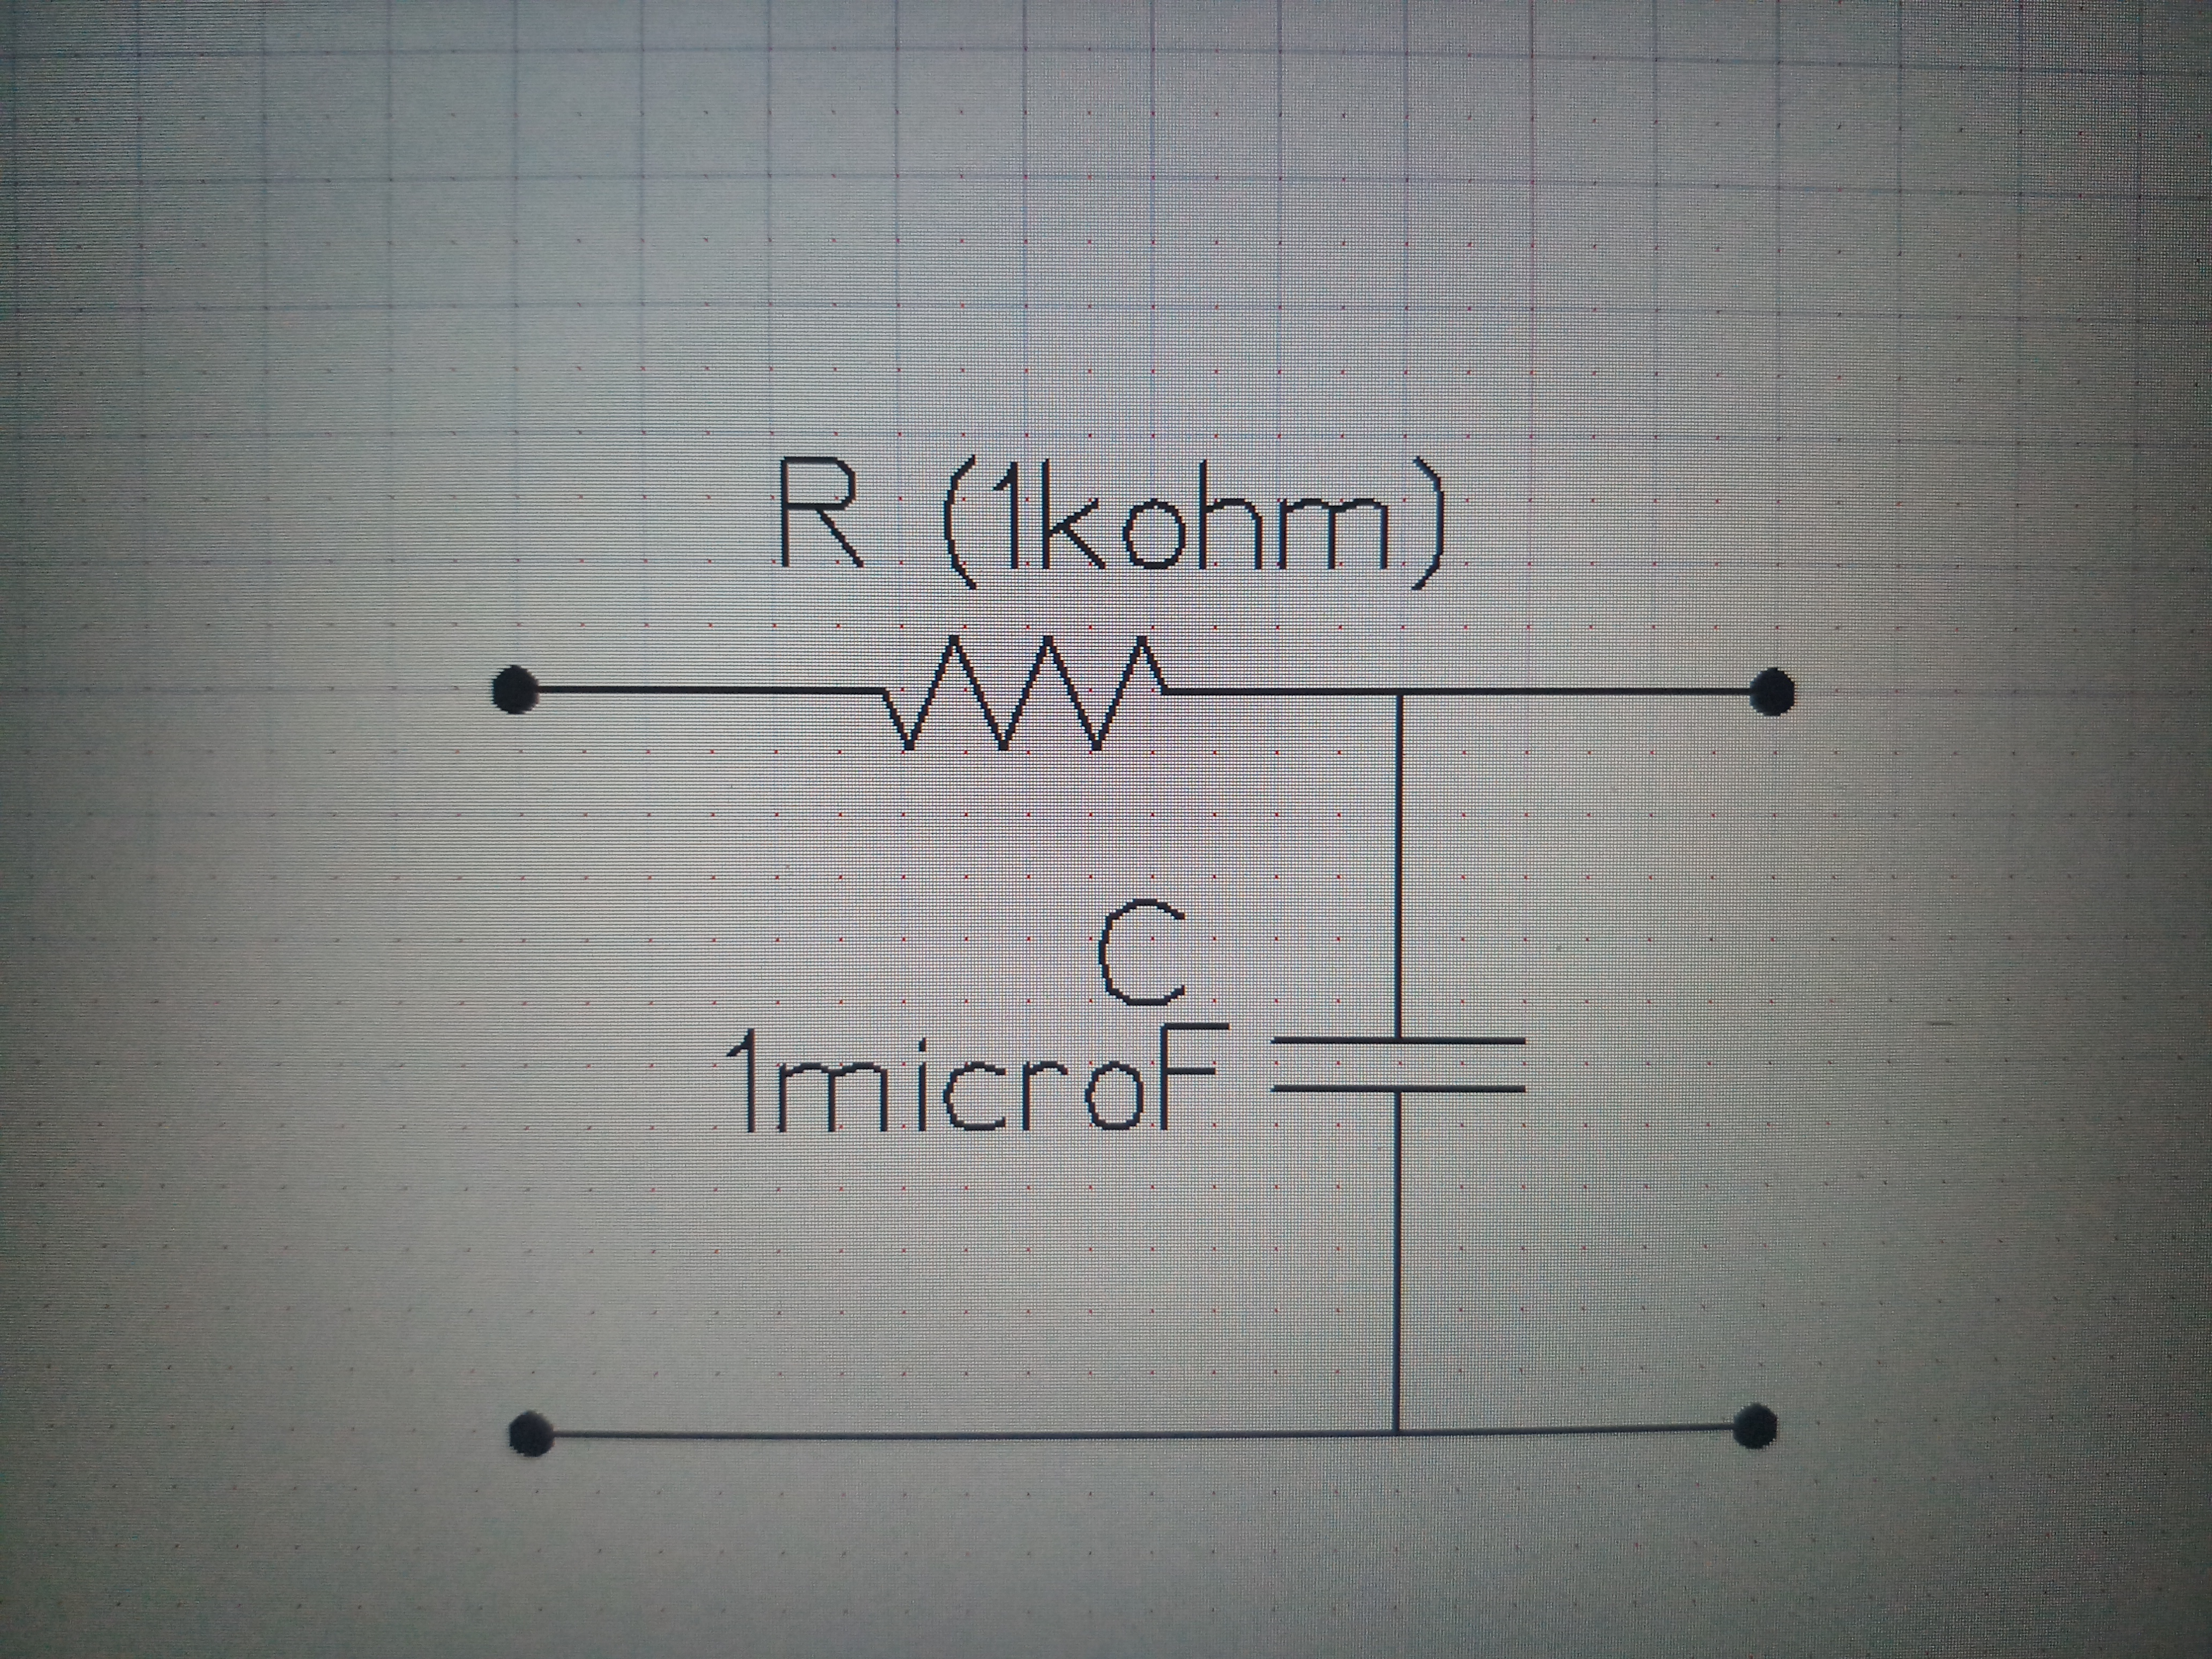
\includegraphics[scale = 0.09]{Circuit_Diagram.jpg}
\end{figure}

\section{Experimental results}
\subsection{Part-1}

The experiment displayed the low-band pass filtering of the RC circuit. Certain graphs have been attached below.
\begin{figure}[h!]

\includegraphics[scale = 0.1]{1.jpg}
\end{figure}


\section{Experiment completion status}
The first part of the experiment was completed, although certain images have not been added in order to avoid redundancies. Part 2 and the simulation have not been completed.

\end{document}
